\section{Conociendo a \textit{Kotest}}
\label{sec:conociendo-kotest}

  Ahora veremos cómo utilizar \idxit{Kotest} para testear nuestras aplicaciones siguiendo una
  metodología de desarrollo basada en pruebas.
  Para esto, comencemos por definir lo más básico de nuestro juego.

  Pero antes, instalaremos un nuevo plugin de \textit{IntelliJ} que nos permitirá sacarle más 
  provecho a \textit{Kotest}.
  Para esto, vayamos a \textit{File} $\rightarrow$ \textit{Settings} $\rightarrow$ \textit{Plugins},
  y busquemos \textit{Kotest} en el \textit{Marketplace}.
  Una vez instalado, \textit{IntelliJ} nos preguntará si queremos reiniciar el IDE, hagámosle caso.

  Cuando desarrollamos aplicaciones, las cosas se pueden complicar muy rápido.
  Es por esto que lo que es muy importante partir siempre por lo más simple.
  En este caso, vamos a comenzar con una clase que represente a un \textit{Bakémon}.
  ¿Pero qué es lo más simple?
  Simple, una clase que represente a un Bakémon sin nigún método ni atributo.
  Así que vamos a comenzar por ahí.

  Primero, busquemos el directorio \url{src/test/kotlin} y creemos un nuevo paquete llamado 
  \url{cl.ravenhill.bakemon}.
  Ahora, dentro de este paquete, creemos una nueva clase llamada \textit{BakemonTest}.
  Aquí es probable que \textit{IntelliJ} nos pregunte si queremos agregar el archivo a \textit{Git},
  esto es equivalente a hacer \textit{git add} en la línea de comandos, así que hagámosle caso.

  Ahora, deberíamos tener una clase que se ve así:

  \begin{kotlin}
    package cl.ravenhill.bakemon

    class BakemonTest {
    }
  \end{kotlin}

  A continuación necesitamos decirle al framework que esta clase es un test.
  Para esto, heredaremos de la clase \textit{FunSpec} de la siguiente forma:

  \begin{kotlin}
    package cl.ravenhill.bakemon

    import io.kotest.core.spec.style.FunSpec

    class BakemonTest : FunSpec({})
  \end{kotlin}

  Algo que notar aquí es que le estamos pasando \texttt{\{\}} como argumento al constructor de la
  clase \textit{FunSpec}.
  Esto se conoce como \textbf{función lambda} y es una forma de pasar un bloque de código como
  argumento a una función o constructor, por ahora no nos preocupemos por esto, más adelante veremos
  en más detalle funciones lambda.

  Ahora vamos a crear nuestro primer test.
  Para esto, primero pensemos en qué es lo que podemos testear de una clase vacía.
  En este caso, lo primero que querremos ver es que el constructor funcione correctamente.
  ¿Pero cómo testeamos que un constructor de una clase vacía funciona correctamente?
  La solución dependerá de la clase que estemos testeando, pero una solución común sería ver que dos
  objetos creados a partir de la misma clase son iguales.
  Lo siguiente es poner en palabras lo que queremos testear, en este caso, podemos decir: 
  \textit{Dos objetos creados a partir de la misma clase deben ser iguales}.
  Una vez hemos planteado nuestro test, podemos agregar ese test a nuestra clase de la siguiente
  forma:

  \begin{kotlin}
    class BakemonTest : FunSpec({
      test("Two objects created from the same class should be equal") {}
    })
  \end{kotlin}

  Y con eso tenemos nuestro primer test.
  Probemos qué sucede si lo ejecutamos.
  Para esto, podemos hacer click al botón \enquote{play} al lado izquierdo de la definición de la
  clase y seleccionando la opción \enquote{Run 'BakemonTest'}.
  Esperamos un poco a que se corran los tests y podemos ver que el test que acabamos de crear pasa
  (\cref{fig:primer-test}).
  ¡Felicidades!
  Tenemos el primer error de este capítulo.

  \begin{figure}[ht!]
    \centering
    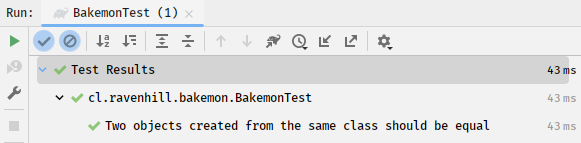
\includegraphics[width=0.5\textwidth]{img/oop/tdd/kotest/kotest_primer_test.png}
    \caption{Primer test}
    \label{fig:primer-test}
  \end{figure}

  Como dijimos antes, el primer paso del TDD es crear un test que falle.
  En este caso es fácil ver por qué nos pasó esto.
  El test que acabamos de crear no tiene ninguna aserción, por lo que siempre va a pasar.
  Solucionar esto es simple, simplemente agreguemos una aserción que verifique que dos objetos
  creados a partir de la misma clase son iguales-
  Para esto, utilizaremos la función \textit{shouldBe} que verifica que dos objetos sean iguales.

  \begin{kotlin}
    test("Two objects created from the same class should be equal") {
      val a = Bakemon()
      val b = Bakemon()
      a shouldBe b
    }
  \end{kotlin}

  Ahora, si tratamos de correr el test recibiremos un error diciendo 
  \enquote{\textit{Unresolved reference: Bakemon}}.
  Esto es porque la clase \textit{Bakemon} no existe.
  Pero lo importante es que esto significa que nuestro test falla.

  \begin{center}
    ¿Yay?
  \end{center}

  Con esto podemos pasar al siguiente paso del TDD, que es crear el código mínimo necesario para que
  el test pase.
  Creemos un paquete \url{cl.ravenhill.bakemon} en el directorio \url{src/main/kotlin} y dentro de
  ese paquete creemos una clase llamada \textit{Bakemon}.
  De nuevo, esto nos creará una clase vacía:

  \begin{kotlin}
    package cl.ravenhill.bakemon

    class Bakemon {
    }
  \end{kotlin}

  Ahora, si corremos el test, veremos que sigue fallando pero con un error distinto.
  En este caso obtendremos lo siguiente:

  \begin{minted}{text}
    expected:<cl.ravenhill.bakemon.Bakemon@4578b1f> 
    but was:<cl.ravenhill.bakemon.Bakemon@27559659>
    Expected :cl.ravenhill.bakemon.Bakemon@4578b1f
    Actual   :cl.ravenhill.bakemon.Bakemon@27559659
    <Click to see difference>
  \end{minted}
  
  ¿Por qué pasa esto?
  ¿No son ambos objetos iguales?
  La respuesta es que sí, pero \textit{Kotlin} no tiene forma de saberlo, ya que no le hemos dicho
  bajo qué criterio dos objetos son iguales.

  Otra cosa que podemos notar es que el error utiliza un nombre poco intuitivo para nuestras clases.
  Esto es lo primero que solucionaremos.
  Puede que ya se hayan dado cuenta de que el nombre que utiliza \textit{Kotest} para nuestros 
  objetos es muy parecido al que vimos en el \cref{sec:method-lookup}, y la causa es la misma: no
  hemos definido un método \idx{\texttt{toString}} para nuestras clases.
  Hagamos eso:

  \begin{kotlin}
    class Bakemon {
      override fun toString(): String {
        return "Bakemon"
      }
    }
  \end{kotlin}

  Ahora, si corremos el test, tendremos un mensaje más amigable:

  \begin{minted}{text}
    expected:<Bakemon> but was:<Bakemon>
    Expected :Bakemon
    Actual   :Bakemon
    <Click to see difference>
  \end{minted}

  Lo siguiente, es decirle a \textit{Kotlin} cómo comparar dos objetos de la clase \textit{Bakemon}.
  Pero para esto entendamos primero qué significa que dos objetos sean iguales.

  En \textit{Kotlin} existen dos maneras de verificar si dos objetos son iguales: igualdad 
  referencial e igualdad estructural.
  
  La \textbf{igualdad referencial}\index{igualdad referencial} se refiere a que dos objetos son 
  iguales si y sólo si ocupan el mismo espacio en memoria.
  Esto significa que si tenemos dos variables que referencian al mismo objeto, entonces esos dos 
  objetos son iguales.
  En \textit{Kotlin}, la igualdad referencial se verifica con el operador \texttt{===}.

  Por otro lado, la \textbf{igualdad estructural} se refiere a que dos objetos son iguales si y sólo
  si los atributos que lo identifican son iguales.
  A diferencia de la igualdad referencial, esta condición debemos definirla nosotrxs.
  En \textit{Kotlin}, la igualdad estructural se verifica con el operador \texttt{==}.
  Existen dos métodos que definen la igualdad estructural en \textit{Kotlin}:

  \begin{itemize}
    \item \texttt{Any::equals(Any?): Boolean} que verifica que dos objetos sean iguales de acuerdo 
      a la igualdad estructural.
    \item \texttt{Any::hashCode(): Int} que retorna un número entero que identifica a un objeto.
      Este número generalmente no lo utilizaremos explícitamente, pero la librería estándar de 
      \textit{Kotlin} espera que si dos objetos son iguales de acuerdo al método \texttt{equals},
      entonces sus códigos de hash deben ser iguales.
  \end{itemize}

  \begin{important}
    Si no definimos la igualdad estructural explícitamente, entonces \textit{Kotlin} utilizará la
    igualdad referencial.
  \end{important}

  \begin{important}
    El método \texttt{shouldBe} espera que dos objetos sean iguales de acuerdo a la igualdad
    estructural.
  \end{important}

  \begin{note}
    El método \texttt{equals} recibe un parámetro de tipo \texttt{Any?} y no de tipo
    \texttt{Any}. 
    \texttt{Any?} es el supertipo de todos los \textbf{tipos} de \textit{Kotlin}, mientras que 
    \texttt{Any} es la superclase de todos los objetos en \textit{Kotlin}.
    Esta diferencia es importante, ya que no todo en \textit{Kotlin} es un objeto, pero no nos
    detendremos en eso por ahora.
  \end{note}

  La igualdad estructural siempre se define de la misma forma:

  \begin{itemize}
    \item Verificar si el objeto con el que estamos comparando es igual referencialmente.
      Esto lo hacemos para mejorar el rendimiento de la comparación.
    \item Verificar si el objeto con el que estamos comparando es de la misma clase.
      Esto lo hacemos porque dos objetos de distinta clase podrían tener los mismos atributos.
    \item Verificar si los atributos que identifican a los objetos son iguales.
  \end{itemize}

  En nuestro caso, la clase \textit{Bakemon} no tiene atributos, por lo que no haremos la tercera
  verificación.
  Traduzcamos esto a código:

  \begin{kotlin}
    override fun equals(other: Any?): Boolean {
      return if (other === this) {
        true
      } else {
        other is Bakemon
      }
    }
  \end{kotlin}

  Ahora, si corremos el test, veremos que pasa.

  Nos falta implementar el método \texttt{hashCode}, pero recuerden que estamos aplicando el TDD,
  por lo que primero debemos crear un test que falle.
  Hagamos eso:

  \begin{kotlin}
    test("Two objects created from the same class should have the same hashCode") {
      val a = Bakemon()
      val b = Bakemon()
      a shouldHaveSameHashCodeAs b
    }
  \end{kotlin}

  Ahora, si corremos el test, veremos que falla.
  Con esto, podemos implementar el método \texttt{hashCode}.
  Como dijimos, el método \texttt{hashCode} debe ser consistente con la igualdad estructural, esto
  significa que debemos considerar qué identifica a un objeto.
  Para esto, revisemos el método \texttt{equals} que acabamos de implementar.
  ¿Qué identifica a un objeto de la clase \textit{Bakemon}?
  Podríamos pensar que nada, ya que no tiene atributos, pero no es así.
  Hay una cosa que identifica a un objeto de la clase \textit{Bakemon}, y es su clase.
  Por lo tanto, podemos implementar el método \texttt{hashCode} de la siguiente forma:

  \begin{kotlin}
    override fun hashCode(): Int {
      return Objects.hash(Bakemon::class)
    }
  \end{kotlin}

  Noten que en lugar de definir nuestra propia manera de calcular el código de hash, estamos
  utilizando la función \texttt{Objects.hash} que está definida en la librería estándar de
  \textit{Kotlin}.

  Ahora, si corremos el test, veremos que pasa.

  Para terminar, haremos \textit{commit} de los cambios que hemos hecho hasta ahora:

  \begin{powershell}
    git add .
    git commit -m "FEAT Adds toString, equals and hashCode to Bakemon"
  \end{powershell}